
\begin{center}
\Huge
Aflevering 6
\end{center}
\section*{Opgave 1}
\stepcounter{section}

I en by er luftpartikelkoncentrationen af en bestemt type udstødningspartikel målt fra år $2000$ til år $2010$. Den målte koncentration (i ppm) som funktion af tiden (i år) kan ses af følgende tabel:
\begin{center}
\begin{tabular}{c|c|c|c|c|c|c|c|c|c|c|c}
$t$  & 0 & 1 & 2 & 3 & 4 & 5 & 6 & 7 & 8 & 9  \\
\hline
$C$  &11.67 & 35.15 & 42.49 & 68.97 & 55.61 & 92.73 & 103.22 & 150.53 & 185.23 & 244.42
\end{tabular}
\end{center}

\begin{enumerate}[label=\roman*)]
\item Vi antager, at sammenhængen mellem tiden $t$ og koncentrationen $C$ er på formen
\begin{align}\label{eq:lin}
C(t) = at+b.
\end{align}
Bestem $a$ og $b$, så denne sammenhæng passer bedst på punkterne. 
\item Lav residualanalyse på denne model og vurdér, om en sammenhængen af typen \eqref{eq:lin} beskriver datasættet godt.
\item En genovervejelse af kilden til denne forurering får os til at tro, at sammenhængen mellem luftpartikelkoncentrationen og tiden er givet ved en eksponentiel sammenhæng i stedet. Lav eksponentiel regression på datasættet og kommentér på resultatet.
\item Lav residualanalyse på den eksponentielle model og sammenlign med den tidligere model. Hvilken model virker til at være mest valid?
\item Bestem residualet for begge modeller i år $2005$.
\item Brug begge modeller til at bestemme partikelkoncentrationen i år 2010.
\item Partikelkoncentrationen var i år 2010 på $317.23$ppm. Hvilken model rammer dette bedst?
\item Brug dine svar på i)-vii) til at vurdere, hvilken af de to modeller, der bedst beskriver partikelkoncentrationen. 
\end{enumerate}


\section*{Opgave 2}
Vi har punkterne $A = (2,k)$, $B =(-4,1)$ og $C = (-1,-1)$.
\begin{enumerate}[label=\roman*)]
\item Bestem $k$, så $\vv{BA}$ og $\vv{BC}$ er orthogonale.
\item Bestem $k$, så $\vv{BA}$ og $\vv{BC}$ er parallelle. 
\item Bestem $k$, så den lille vinkel mellem $\vv{BA}$ og $\vv{BC}$ er $30^\circ$
\end{enumerate}

\section*{Opgave 3}
Betragt andengradspolynomierne $f$, $g$ og $h$ på Fig. \ref{fig:poly}
\begin{figure}[H]
\centering
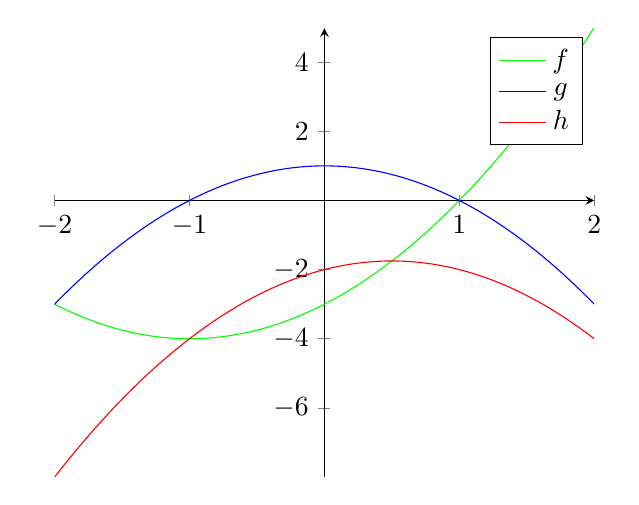
\begin{tikzpicture}
\begin{axis}[axis lines = middle, xmin = -2, xmax = 2, ytick = {}, xtick = {}]
\addplot[samples = 1000, color = green] {x^2+2*x-3};
\addplot[samples = 1000, color = blue] {-x^2+1};
\addplot[samples = 1000, color = red] {-x^2+x-2};
\legend{$f$, $g$, $h$}
\end{axis}
\end{tikzpicture}
\caption{Polynomier}
\label{fig:poly}
\end{figure}
\begin{enumerate}[label=\roman*)]
\item Bestem fortegnene for koefficienterne $a,$ $b$ og $c$ for $f$, $g$ og $h$ ved at betragte Fig. \ref{fig:poly}. Begrund dit svar.
\item Bestem fortegnet på diskriminanten for $f$, $g$ og $h$. Begrund dit svar. 
\end{enumerate}

\section*{Opgave 4}
Et mål for sundhed hos både mænd og kvinder er det såkaldte BMI (Body Mass Index). BMI for en person bestemmes som
\begin{align*}
f(h,m) = \frac{m}{h^2},
\end{align*}
hvor $h$ er højde i meter og $m$ er vægt i $kg$. Man betegnes som normalvægtig, hvis man har en BMI i intervallet $[18.5,25]$. 
\begin{enumerate}
\item Gennemsnitshøjden for danske kvinder var i 2005 167cm og gennemsnitsvægten var 68kg. Hvad er BMI for gennemsnitskvinden?
\item Hvis en person på 167cm skal være normalvægtig, hvad er så det højeste, hun må veje? Hvad med det laveste?
\item Rekorden for højeste vægt har amerikaneren Jon Brower Minnoch. Han havde, da han var tungest en BMI på 185.5, og han var 185cm høj. Hvad vejede han?
\item Hvor mange kg skulle Jon tabe for at blive normalvægtig?
\end{enumerate}

\section*{Opgave 5}
En eksponentialfunktion
\begin{align*}
f(x) = 1.3\cdot (1.05)^x
\end{align*}
er givet. 
\begin{enumerate}[label=\roman*)]
\item Bestem $f(10)$.
\item Løs ligningen $f(x) = 2$.
\item Hvad er fordoblingskonstanten for $f$?
\end{enumerate}
